\section{Data Analysis} \label{data}
At the time of writing, 274 participants have played the game.

\subsection{Demographics}
As stated previously, the game was mainly shared on gaming websites. Tables \ref{table:demographics1} and \ref{table:demographics2} show demographical data about the participants. Most of the participants rated themselves rather experienced with both playing videogames in general and playing 2D platforming games.


%%% This is how to insert a table %%%
\begin{table}[htbp]
\scriptsize
\centering
\begin{tabular}{|l|l|l|l|}
\hline
\textbf{Platform} & Windows Web & Windows Exe & Mac Web \\
                  & 55,2\%      & 30,7\%      & 14,1\%  \\
\hline
\textbf{Gender}   & Male        & Female      & Other   \\
                  & 93,6\%      & 5,7\%       & 0,7\%   \\
\hline
\textbf{Averages}      & Age     & Framerate            & Time spent        \\
                  & 24,6 years  & 59,7 FPS           & 61 seconds/level        \\
\hline
\end{tabular}
\caption{Demographics data 1.}
\label{table:demographics1}
\end{table}


tex text text


\begin{table}[h]
\scriptsize
\centering
\begin{tabular}{|l|ll|}
\hline
\textbf{Region}                      &                & \textbf{}               \\ \hline
\textit{Europe}                      & 70,6\%         &                         \\ \hline
\textit{Americas}                    & 26,7\%         &                         \\ \hline
\textit{Asia}                        & 1,9\%          &                         \\ \hline
\textit{Oceania}                     & 0\%            &                         \\ \hline
\textit{Africa}                      & 0,6\%          &                         \\ \hline
\textit{Other}                       & 0,2\%          &                         \\ \hline
\textit{\textbf{Experience with...}} & \textbf{Videogames} & \textbf{2D platformers} \\ \hline
\textit{1 (none)}                           & 0\%            & 0\%                     \\ \hline
\textit{2}                           & 0\%            & 3,1\%                   \\ \hline
\textit{3}                           & 0,6\%          & 10,1\%                  \\ \hline
\textit{4}                           & 4\%            & 14,1\%                  \\ \hline
\textit{5}                           & 9,6\%          & 23,2\%                  \\ \hline
\textit{6}                           & 22,5\%         & 16,9\%                  \\ \hline
\textit{7 (a lot)}                           & 63,3\%         & 32,6\%                  \\ \hline
\end{tabular}
\caption{Demographics data 2.}
\label{table:demographics2}
\end{table}


As stated in Section \ref{latinSection}, ideally there should be an equal amount of participants in each of the four Latin square sequences. However, as shown in Table \ref{table:latinSequenceNumber}, this is not the case. This might be due to either players quitting halfway, or that participants for some reason lost the Internet connection while trying to access the current Latin square number (in this case, the sequence was chosen randomly). The average number of completed levels were 2,5 per participant. This might be due to the fatigue mentioned in Section \ref{latinSection}. 274 have begun the game, i.e., playing the first level after the two anchoring examples mentioned in Section \ref{task}. Each time a participant collects three stars and answer the questionnaire, data is logged. In total, there were 701 data logs. Figure \ref{fig:retention} illustrates the retention rate of the participants.

%%% This is how to insert a table %%%
\begin{table}[htbp]
\scriptsize
\centering
\begin{tabular}{|c|c|}
\hline
 & \textbf{\# of participants}\\
 \hline
\textbf{Sequence 1} & 190\\
\hline
\textbf{Sequence 2} & 179\\
\hline
\textbf{Sequence 3} & 165\\
\hline
\textbf{Sequence 4} & 167\\
\hline
\end{tabular}
\caption{The number of participants in each of the four Latin square sequences.}
\label{table:latinSequenceNumber}
\end{table}

\begin{figure}[htbp]
\centering
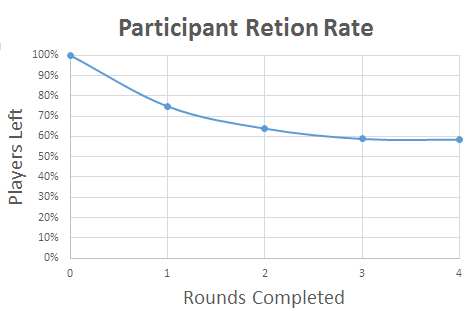
\includegraphics[width=0.4\textwidth]{Pics/retetionRate}
\caption{Due fatigue or other factors, not all participants played the four rounds.}
\label{fig:retention}
\end{figure}


